\chapter{Liquid Dynamics}

A non-circularly symmetric molecule on a plane has three degrees of freedom, translations in the $x$ and $y$ directions and a rotation in the $xy$ plane. Understanding the dynamics of a system requires an understanding of the translations and rotations that take place within that system, providing a basis for further study and giving information about the timescales on which events are likely to occur.

\section{Choice of Molecules}

To choose the molecules that we are studying in depth in this thesis, a survey of a wide range of molecular shapes was conducted. The survey included both the Snowman and Trimer molecule types over a radius range $r = [0.5,1]$, a distance range of $d = [1,1+r]$ and an angle range of $\theta = [90^\circ,180^\circ]$. These ranges were chosen so the resulting molecules are sufficiently distinct from a disc, a problem that has been studied for a long time~\cite{verlet:67}.

\begin{figure}
    \begin{subfigure}{0.5\textwidth}
        \centering
        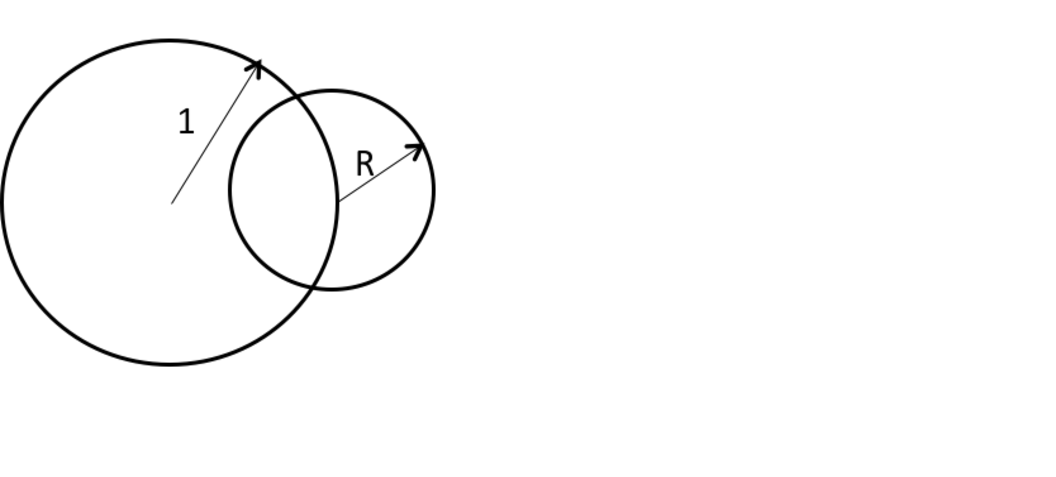
\includegraphics[width=\linewidth]{Snowman}
        \caption{Construction of Snowman molecules}
        \label{fig:snowman}
    \end{subfigure}
    \begin{subfigure}{0.5\textwidth}
        \centering
        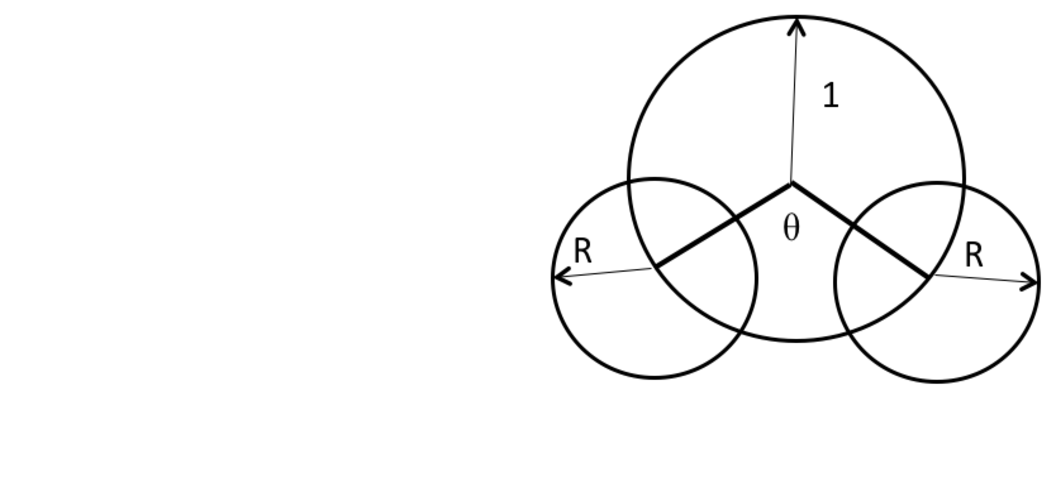
\includegraphics[width=\linewidth]{Trimer}
        \caption{Construction of Trimer molecules}
        \label{fig:trimer}
    \end{subfigure}
    \caption{Construction of the molecules used in this thesis}
    \label{fig:construction}
\end{figure}

The resulting collection of 50 molecules was cooled from a partially randomly generated high temperature state, resulting in a low temperature structure distinct from the initial state. These low temperature structures were assessed for suitability on a number of criteria:
\begin{itemize}
    \item The molecules have to be resistant to crystallisation allowing long time dynamics to be characterised. There had to be no evidence of crystallisation in the low temperature structures.
    \item The molecules have to be radially definable.
    \item The concavity of the molecules should cover a wide range,
    \item The molecules have to be similar enough for direct comparison, and
    \item The molecules are representative of a wide range of molecular shapes.
\end{itemize}
The radius of 0.637556 is interesting as when combined with particles of radius $1.0$ it can form a compact packing. A molecule with a small radius of 0.637556 and a distance between the molecular centers of 1.637556 (\scon) has a crystal structure that mirrors this compact packing. Despite \scon having this low energy crystal structure, the low temperature state exhibited none of this crystal, indicating it is resilient to crystal formation. Retaining a radius of 0.637556 for the other molecules allows a more direct comparison, any differences are due to properties of the arrangement of particles, their shape, rather than the size ratios of the constituent particles. The distance of 1.0 was chosen for both the \tri and \sone, for both consistency between the molecules and to allow all molecules to be described radially. The radial description allows the use of an isopointal search algorithm developed by \textcite{hudson:10} to find the best packing structures as an approximation of the lowest energy structures.

\begin{figure}
    \centering
    \captionsetup{justification=centering}
    \begin{subfigure}[t]{0.3\textwidth}
        \includegraphics[width=\linewidth]{{{Sone}}}
        \caption{$r=0.637556,$\\$d=1.0$ \\\sone}
        \label{fig:sone}
    \end{subfigure}
    \begin{subfigure}[t]{0.3\textwidth}
        \includegraphics[width=\linewidth]{{{Scon}}}
        \caption{$r=0.637556,$\\$d=1.637556$ \\\scon}
        \label{fig:scon}
    \end{subfigure}
    \begin{subfigure}[t]{0.3\textwidth}
        \includegraphics[width=\linewidth]{{{Tri}}}
        \caption{$r=0.637556,$\\$d=1.0, \theta=120 $\\\tri}
        \label{fig:tri}
    \end{subfigure}
    \caption[Molecules chosen for further study]{The molecules chosen for study in this thesis in order of the size of the concavity. The \sone with the smallest concavity, \scon with the smaller disc contacting the large disc and \tri which is a very similar to the \sone molecule.}
    \label{fig:my mols}
\end{figure}

\section{Dynamics of \sone}

\begin{figure}
    \centering
    \begin{subfigure}[t]{0.48\linewidth}
        \includegraphics[width=\textwidth]{{{Snowman-0.637556-1.0-msd}}}
        \caption{MSD, the translational motion}
        \label{fig:snowman 0.637556 1.0 msd}
    \end{subfigure}
    \begin{subfigure}[t]{0.48\linewidth}
        \includegraphics[width=\textwidth]{{{Snowman-0.637556-1.0-C_1}}}
        \caption{C$_1$, the rotational motion}
        \label{fig:snowman 0.637556 1.0 r1}
    \end{subfigure}
    \begin{subfigure}{0.48\textwidth}
        \includegraphics[width=\textwidth]{{{Snowman-0.637556-1.0-F}}}
        \caption{Structure Function, a combination both translations and rotations.}
        \label{fig:snowman 0.637556 1.0 structure}
    \end{subfigure}
    \caption{The main dynamical features of the \sone molecule over a range of temperatures, from a highly mobile liquid to the slowest dynamics we could measure.}
    \label{fig:snowman 0.637556 1.0}
\end{figure} 

With the main dynamical quantities of interest being the translation of the center of mass (COM) and the rotation. The measure of translational motion we are interested in is Mean Squared Displacement (MSD) a measure of the translational motion, the slope of which is related to the diffusion constant. The MSD is given by
\begin{equation}
    MSD(t) = \langle (x(t) - x_0)^2 + (y(t) - y_0)^2 \rangle
\end{equation}
where $x(t)$ and $y(t)$ are the coordinates of the COM at time $t$, while $x_0$ and $y_0$ are the initial coordinates of the molecule while the angle brackets $\langle\,\rangle$ denote averaging over all molecules. The MSD for \sone over a range of temperatures is shown in \textfigref{snowman 0.637556 1.0 msd}. The initial region up to approximately $10^1$ timesteps is the ballistic region where the particles are yet to collide with each other and are moving away from their initial position. At higher temperatures the transition from the ballistic to the diffusive regime is seamless. The diffusive regime is defined by a MSD that increases as a linear function of $t$, indicated by the grey line, where the molecules are rearranging randomly. At lower temperatures like \num{0.90} (shown in red) there is a distinct levelling off of the MSD between the ballistic and diffusive regimes. This region with a slow increase in the MSD is where there are only a small number of molecules that have escaped their local minima, most molecules still have the neighbours that they started with and are vibrating within the bounds of those neighbours.

The second dynamic quantity we are interested in is the rotational relaxation, a measure of the angular mobility of the molecule. The rotational relaxation $C_n(t)$ is given by
\begin{equation}
    C_n(t) = \langle P_n[\vect{e}(0) \cdot \vect{e}(t)] \rangle
\end{equation}
where $P_n$ is the $n$\textsuperscript{th} order Legendre polynomial, $e(t)$ is the orientation vector at time $t$ and the angle brackets $\langle\,\rangle$ denote the averaging over all molecules. The rotational relaxation in this form is a function with a range of $[-1,1]$, a value of $C_n(t)=1$ is when the molecule is in the same orientation as at $t=0$, a value of $C_n(t)=0$ is when the molecule is perpendicular to its initial orientation, and a value $C_n(t)=-1$ when the orientation is perpendicular to the initial orientation\tofix. We are primarily concerned with $C_1$ in which the Legendre polynomial takes the form
\begin{equation}
    P_1(x) = x
\end{equation}
however we do use the second order function $C_2$ later in this thesis for comparison to elucidate further information about rotations. The second order Legendre polynomial is given by
\begin{equation}
    P_2(x) = 2x^2 - 1
\end{equation}

The rotational relaxation for \sone is given in \textfigref{snowman 0.637556 1.0 r1}. The rotational relaxation shows many features that are similar to the MSD, the initial period up to \num{e2} timesteps where the molecules have not had enough time to relax. Once past this initial region higher temperatures show qhich relaxation, however like the MSD at low temperatures there is a stagnation of the relaxation before taking the same shape as the high temperature relaxation. This shape is important in that it is an exponential decay which can be easily characterised.

The third dynamical quantity that we were interested in is the Structure Function $F(t)$. The Structure function is different from the MSD and Rotational relaxations in that instead of calculating quantities for each molecule and averaging over all molecules, the values are calculated for each particle of each molecule and averaged over all the particles. The Structure function is given by
\begin{align}
    F(t) = \left \langle \begin{cases}
        \quad0 &\text{if } \Delta \vect x > 0.3 \\
        \quad1 &\text{if } \Delta \vect x \leq 0.3
    \end{cases} \quad \right \rangle
\end{align}
where $\Delta \vect x$ is the distance of each particle from its initial position and the angle brackets $\langle\,\rangle$ denote averaging over all particles. The value of \num{0.3} was chosen to be small enough to be able to observe the combination of translational and rotational relaxations within a molecule.

The Structure function for \sone is shown in \textfigref{snowman 0.637556 1.0 structure} and shows some interesting characteristics. The initial region between \num{e0} and \num{e1} timesteps is flat as the particles have not had enough time to move a distance of \num{0.3} units. The sharp dropoff, characteristic of the binary function, matches closely with the time that the MSD transitions from the ballistic regime indicative of the molecules escaping their local environment. The other interesting feature is the increase in the Structure function for low temperatures at \num{e4}. This can be explained by the molecular vibrations or rotations of molecules within their initial local environment. Particles will move outside the cutoff distance as part of a vibration and return to their initial positions resulting in the periodicity of the vibrations.

\section{Dynamics of \scon and \tri}

The dynamics of the \scon \figref{scon dynamics} and \tri~\figref{tri dynamics} molecules show similar behaviour to the \sone molecule. The most noticeable difference is the temperature at which the dynamics slow down, in the \sone molecule we are able to collect dynamic quantities down to a temperature of \num{0.50}, for the \scon molecule we are only able to get results down to \num{1.50} and the \tri molecule down to \num{1.05}. We are unable to characterise the dynamics below these temperature as dynamical quantities are not definable where there is no motion of the molecules. The dramatic change in low temperature behaviour for relatively small changes in molecular shape is a result that we investigate further throughout the rest of this thesis.

Apart from the dramatic differences in temperature the dynamics exhibits very similar behaviour. The MSD \figref{snowman 0.637556 1.637556 msd} shows the same levelling out at low temperature in the region between the short time ballistic regime and the long time diffusive regime. The rotational relaxations \figref{snowman 0.637556 1.637556 r1} occur on a longer timescale than \sone as might be expected of the elongated \scon molecule. The Structure function also shows the same behaviour, with peaks which we believe to be a result of the vibrational motion of particles at low temperature.


\begin{figure}
    \centering
    \begin{subfigure}{0.45\linewidth}
        \includegraphics[width=\textwidth]{{{Snowman-0.637556-1.637556-msd}}}
        \caption{MSD}
        \label{fig:snowman 0.637556 1.637556 msd}
    \end{subfigure}
    \begin{subfigure}{0.45\linewidth}
        \includegraphics[width=\textwidth]{{{Snowman-0.637556-1.637556-C_1}}}
        \caption{C$_1$}
        \label{fig:snowman 0.637556 1.637556 r1}
    \end{subfigure}
    \begin{subfigure}{0.45\textwidth}
        \includegraphics[width=\textwidth]{{{Snowman-0.637556-1.637556-F}}}
        \caption{Structure function}
        \label{fig:snowman 0.637556 1.637556 structure}
    \end{subfigure}
    \caption{The dynamics of the \scon molecule over a range of temperatures.}
    \label{fig:scon dynamics}
\end{figure}

\begin{figure}
    \centering
    \begin{subfigure}{0.45\linewidth}
        \includegraphics[width=\textwidth]{{{Trimer-0.637556-1.00-120-msd}}}
        \caption{MSD}
        \label{fig:trimer 0.637556 1.0 120 msd}
    \end{subfigure}
    \begin{subfigure}{0.45\linewidth}
        \includegraphics[width=\textwidth]{{{Trimer-0.637556-1.00-120-C_1}}}
        \caption{C$_1$}
        \label{fig:trimer 0.637556 1.0 120 r1}
    \end{subfigure}
    \begin{subfigure}{0.45\textwidth}
        \includegraphics[width=\textwidth]{{{Trimer-0.637556-1.00-120-F}}}
        \caption{Structure function}
        \label{fig:trimer 0.637556 1.0 120 structure}
    \end{subfigure}
    \caption{Dynamics of the \tri molecule across a range of temperatures.}
    \label{fig:tri dynamics}
\end{figure}


\section{Comparison of Dynamic Quantities}

The functions that we have dealt with so far allow a comparison of the behaviour of a molecule over a range of temperatures, what we are unable to do is easily compare molecules and be able to interpret all the data on a single plot. To make comparisons we want to represent each function as a single value. From the MSD the diffusion constant can be found by
\begin{equation}
    D = \frac{1}{4}\ddiff{\,MSD(t)}{t}
\end{equation} 
a multiple of the gradient. The gradient of the MSD from which the diffusion constant is defined is in the diffusive region. To calculate an accurate value of the diffusion constant an average value of the gradient was calculated for this region. The rotational relaxation and the structure function are similar in nature and can be treated in the same way. We can define relaxation times $\tau_1,\tau_2,\text{and},\tau_s$ as the time for these functions to reach a specific value. The exponentially decaying nature of the rotational relaxation and structure functions makes the value of $1/\e$ relevant since at that point the time $t$ is related to the exponential factor $k$ by the relation $k=1/t$.

\begin{figure}
    \centering
    \begin{subfigure}{0.6\linewidth}
        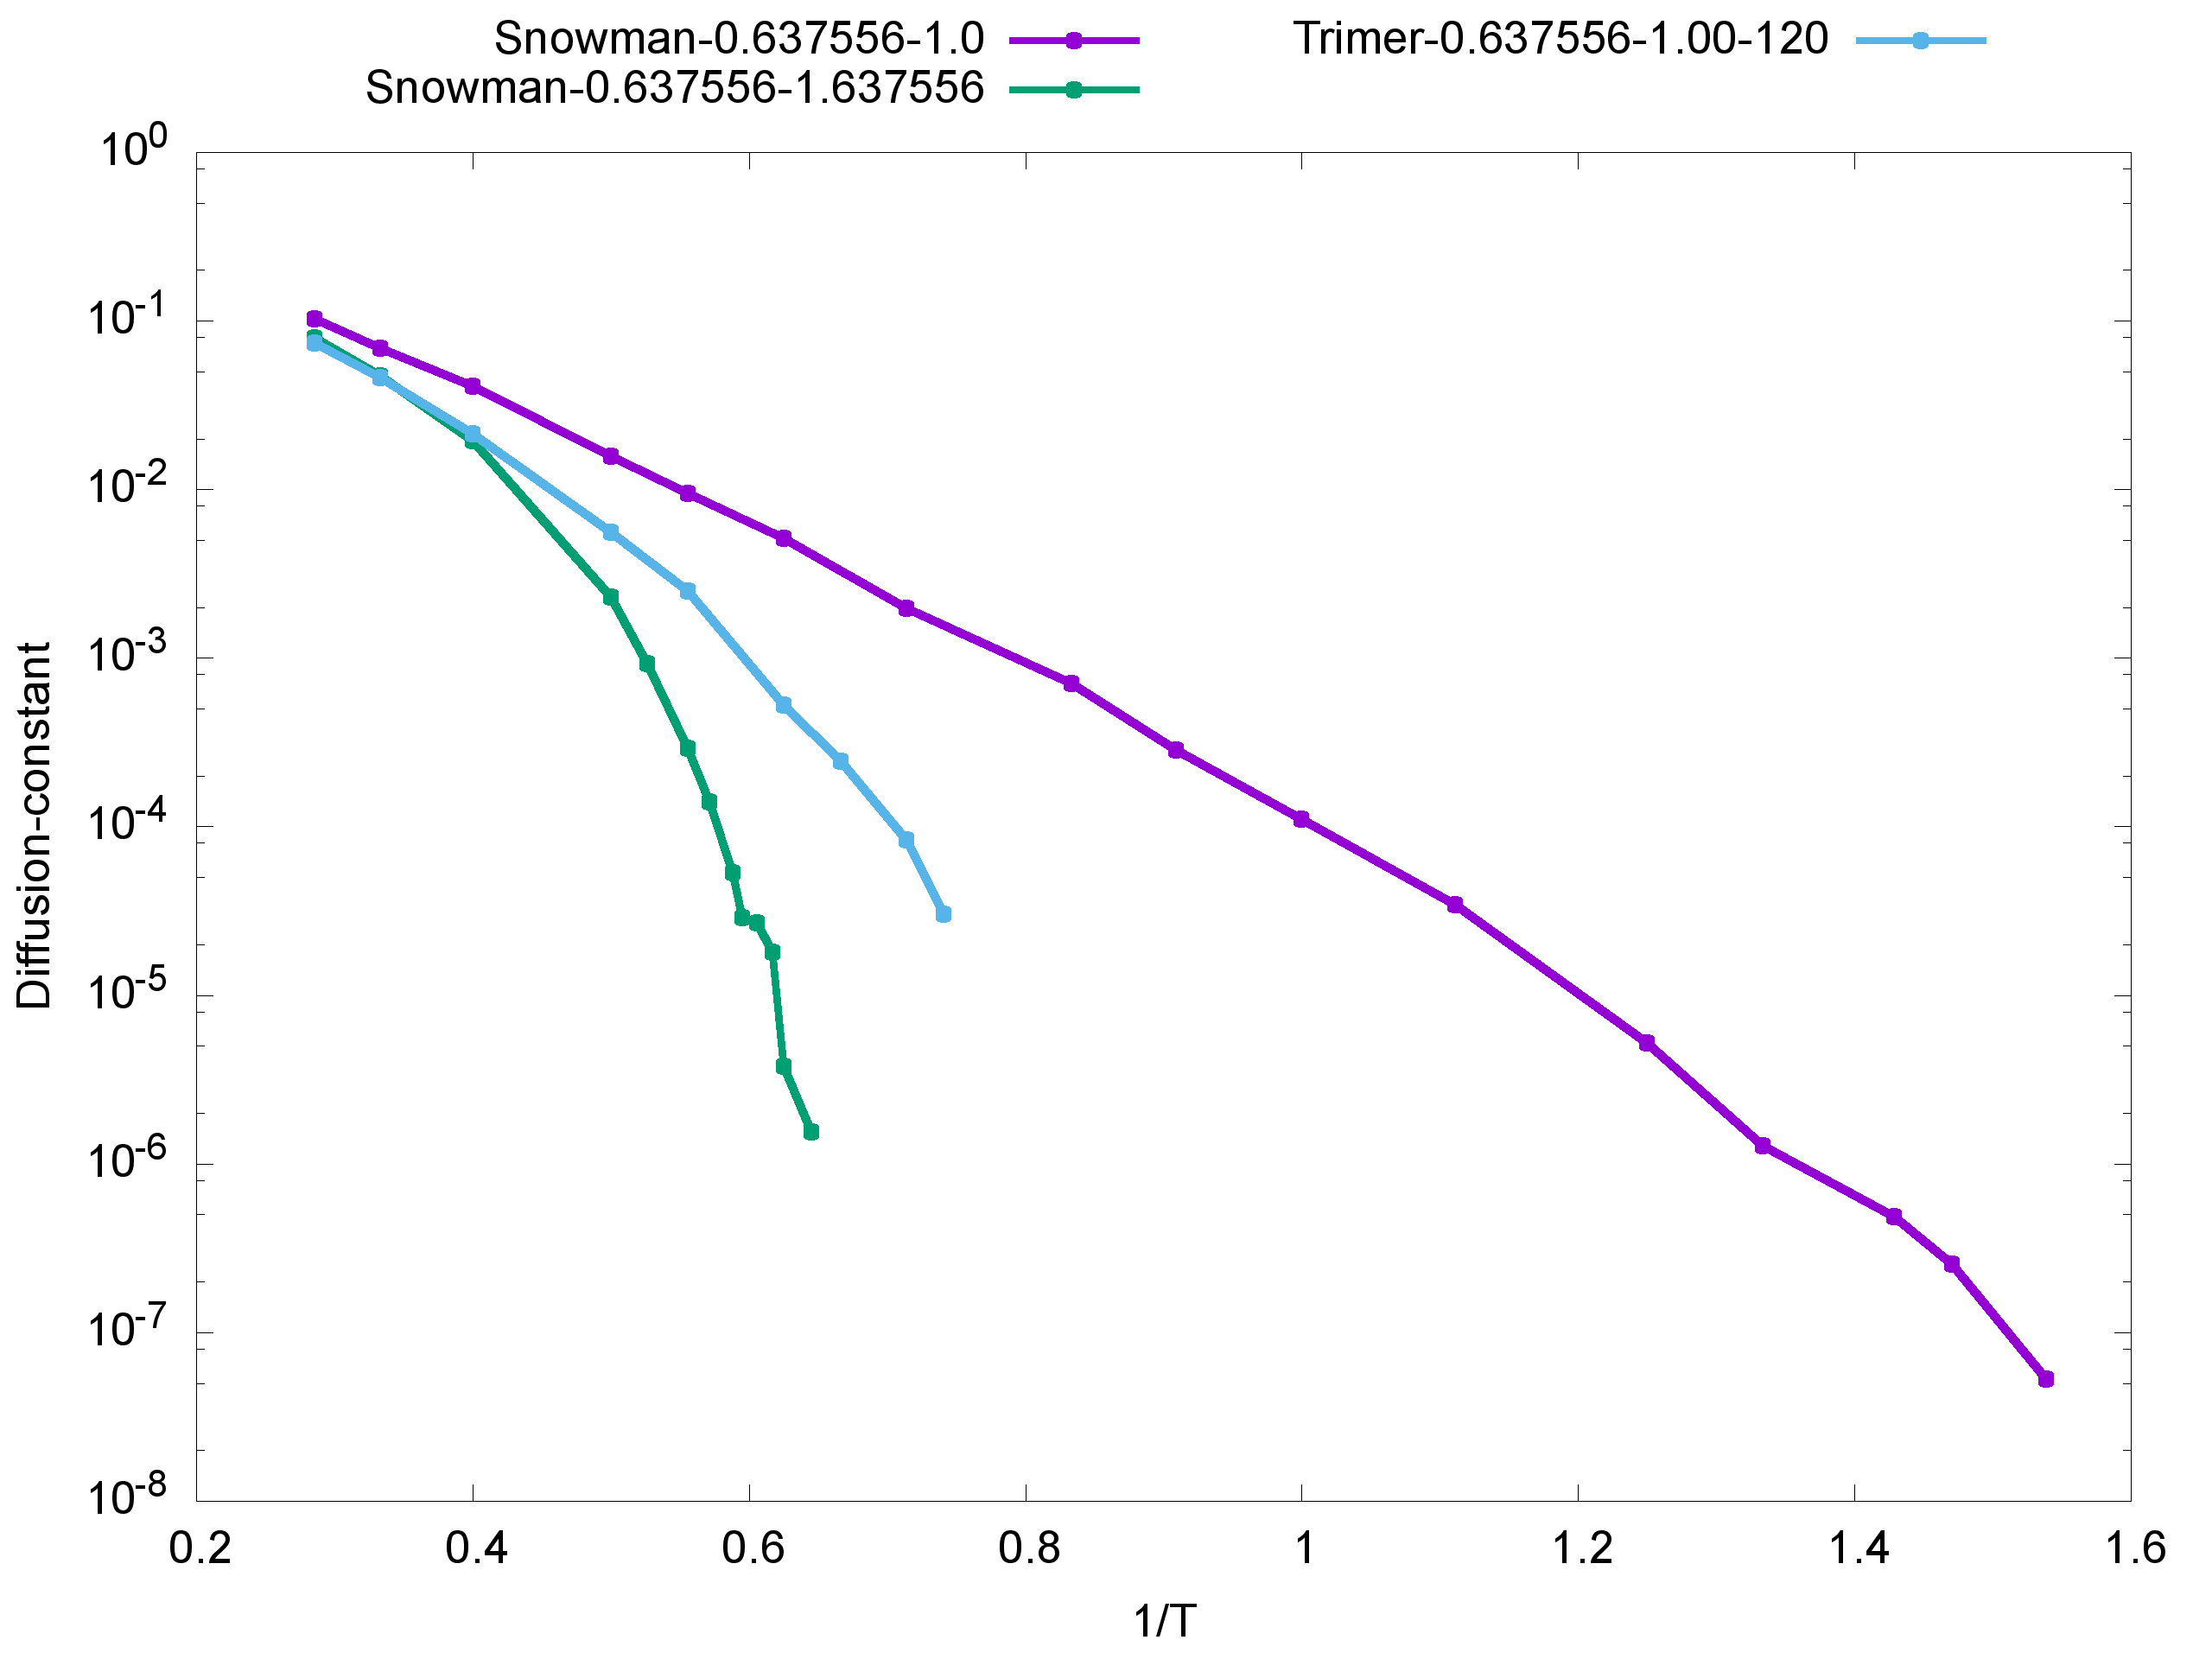
\includegraphics[width=\textwidth]{Diffusion-constant}
        \caption{The \sone molecule displays a diffusion constant that is fairly linear, while the small change in shape of the \scon molecule results in a dramatic decrease in the diffusion constant.}
        \label{fig:diffusion constant}
    \end{subfigure}
    \begin{subfigure}{0.6\linewidth}
        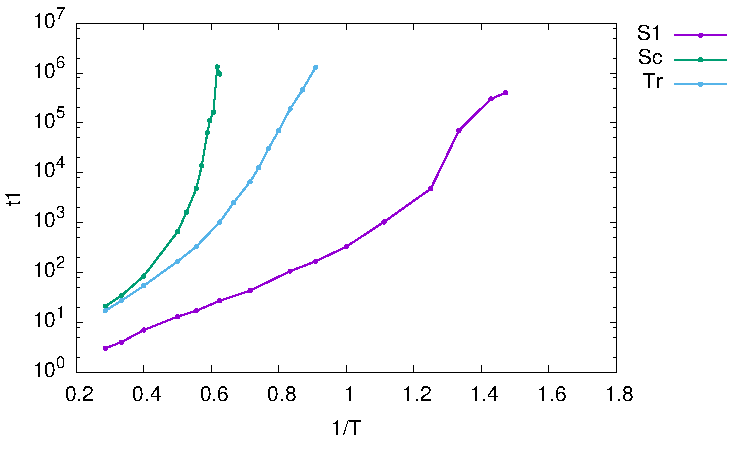
\includegraphics[width=\textwidth]{t1}
        \caption{Somewhat counter intuitively the larger \tri molecule has a faster rotational relaxation than the \scon molecule.}
        \label{fig:tau1}
    \end{subfigure}
    \begin{subfigure}{0.6\textwidth}
        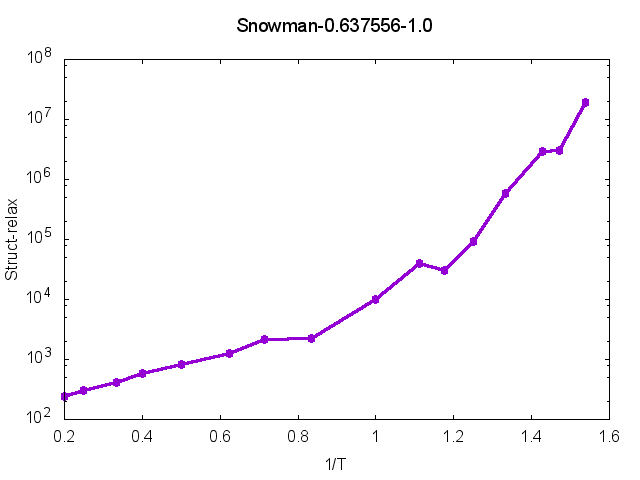
\includegraphics[width=\textwidth]{struct-relax}
        \caption{The difference in fragility of these systems is immense, the \sone molecule displays moderate fragility, the \tri molecule is a fragile system while the \scon molecule is phenomenally fragile spanning five decades of $\tau_s$ over a small temperature range.}
        \label{fig:struct relax}
    \end{subfigure}
    \caption{Comparison of the diffusion constant, rotational relaxation time $\tau_1$ and structural relaxation time $\tau_s$ for the three molecules that we are studying. The small differences in shape result in behaviour differing by many orders of magnitude.}

    \label{fig:dynamic comparison}
\end{figure}

From \textfigref{diffusion constant} we can see that the fragility increases from \sone to \tri to \scon. This suggests that molecular shape is one of the features responsible for the fragility and by extension the formation of the glassy phase. Along with the temperature dependence of these dynamic quantities we often want to know the relative contribution of the various components to the overall dynamics. Taking the product of the diffusion constant $D$ with the rotational relaxation time $\tau_1$ we get the relationship in~\textfigref{D.t1}. The decrease of this function for the \tri molecule as the temperature drops indicates the diffusion constant is decreasing faster than the rotational relaxation is growing; at low temperatures the molecules are more rotationally mobile than translationally mobile. The increasing contribution of the rotation to the dynamics is behaviour observed in previous research. What has not been observed however is the large spike at the lowest temperatures of the \sone and \scon molecules where the translational diffusion is once again far more present in the overall dynamics than the rotations. The sudden spike is a result of an increase in the rotational relaxation time.


\begin{figure}
    \begin{subfigure}{0.5\textwidth}
        \includegraphics[width=\textwidth]{{{D.t1}}}
        \caption{}
        \label{fig:D.t1}
    \end{subfigure}
    \begin{subfigure}{0.5\textwidth}
        \includegraphics[width=\textwidth]{{{D.ts}}}
        \caption{}
        \label{fig:struct relax}
    \end{subfigure}
    \caption{Product of the diffusion constant with relaxation times.}
\end{figure}

\begin{figure}
    \begin{subfigure}{0.5\textwidth}
        \includegraphics[width=\textwidth]{{{t1.t2}}}
        \caption{The ratio of $\tau_1$ to $\tau_2$}
        \label{fig:t1/t2}
    \end{subfigure}
    \begin{subfigure}{0.5\textwidth}
        \includegraphics[width=\textwidth]{{{t1.ts}}}
        \caption{Structural relaxation times}
        \label{fig:struct relax}
    \end{subfigure}
    \caption{Combination of dynamic quantities}
\end{figure}

We hypothesise that the large differences in the dynamical quantities are a result of the local interactions of the molecules. We can test this hypothesis using the Debye-Waller factor. 

\begin{figure}
    \centering
    \begin{subfigure}{0.45\linewidth}
        \includegraphics[width=\textwidth]{{{Snowman-0.637556-1.0-dMSD}}}
        \caption{}
    \end{subfigure}
    \begin{subfigure}{0.45\linewidth}
        \includegraphics[width=\textwidth]{{{Snowman-0.637556-1.637556-dMSD}}}
        \caption{}
    \end{subfigure}
    \begin{subfigure}{0.45\textwidth}
        \includegraphics[width=\textwidth]{{{Trimer-0.637556-1.00-120-dMSD}}}
        \caption{}
    \end{subfigure}
    \caption{Taking the slope of the MSD as plotted in the MSD plots, log, log}
    \label{fig:tri dynamics}
\end{figure}

\begin{figure}
    \centering
    \includegraphics[width=\textwidth]{{{logD.DW}}}
    \caption{Plotting the diffusion constant against Debye-Waller factor we get all molecules on the same line.}
\end{figure}

\section{Dynamic Inhomogeneities}

All the properties we have investigated so far have been averages over all the molecules or particles. These properties are geared towards homogeneous liquids, where all molecules show similar behaviour. One of the features of supercooled liquids is inhomogeneous dynamics, where the dynamics of the system is dominated by a small number of highly mobile molecules. One measure of the homogeneity of the system is the nongaussian parameter $\alpha(t)$ a measure of how closely the MSD of the system matches that of a gaussian distribution, the distribution a high temperature liquid would match. The nongaussian parameter is given by
\begin{equation}
    \alpha(t) = \frac{\langle \Delta x(t)^4 \rangle}{2 \langle \Delta x(t)^2\rangle^2} - 1
\end{equation}
where $\Delta x(t) = \sqrt{(x(t) - x_0)^2 + (y(t) - y_0)^2}$ and the angle brackets $\langle\,\rangle$ denote averaging over all molecules.

\begin{figure}
    \centering
    \includegraphics[width=0.5\linewidth]{{{Trimer-0.637556-1.00-120-alpha}}}
    \caption{Nongaussian function}
    \label{fig:tri alpha}
\end{figure}

The nongaussian parameter for \tri is given in \textfigref{tri alpha}. We can see that that with decreasing temperature there is an increase in the nongaussian parameter, meaning an increase in the dynamic inhomogeneities. There is also a move of the peak of the dynamic inhomogeneities to longer timescales as the temperature increases, a result that matches previous observations.

\begin{figure}
    \centering
    \includegraphics[width=0.5\linewidth]{{{Trimer-1.15-0.637556-1.00-120-moved}}}
    \caption{Movement of particles within a frame. This shows the net motions of all \sone molecules over a simulation run. The motion of the centers of mass are displayed by the vectors, directly representing the motion that took place. The magnitude of the rotation is given by the intensity of the green circles.}
    \label{fig:}
\end{figure}

